The PMT box (Fig. \ref{fig:laspmtbox}) comprehends two PMTs \cite{ref:pmt} used to trigger the \lasii~acquisition in the \laser~mode. It houses two electronic boards :


\begin{figure}[htbp]
\centering
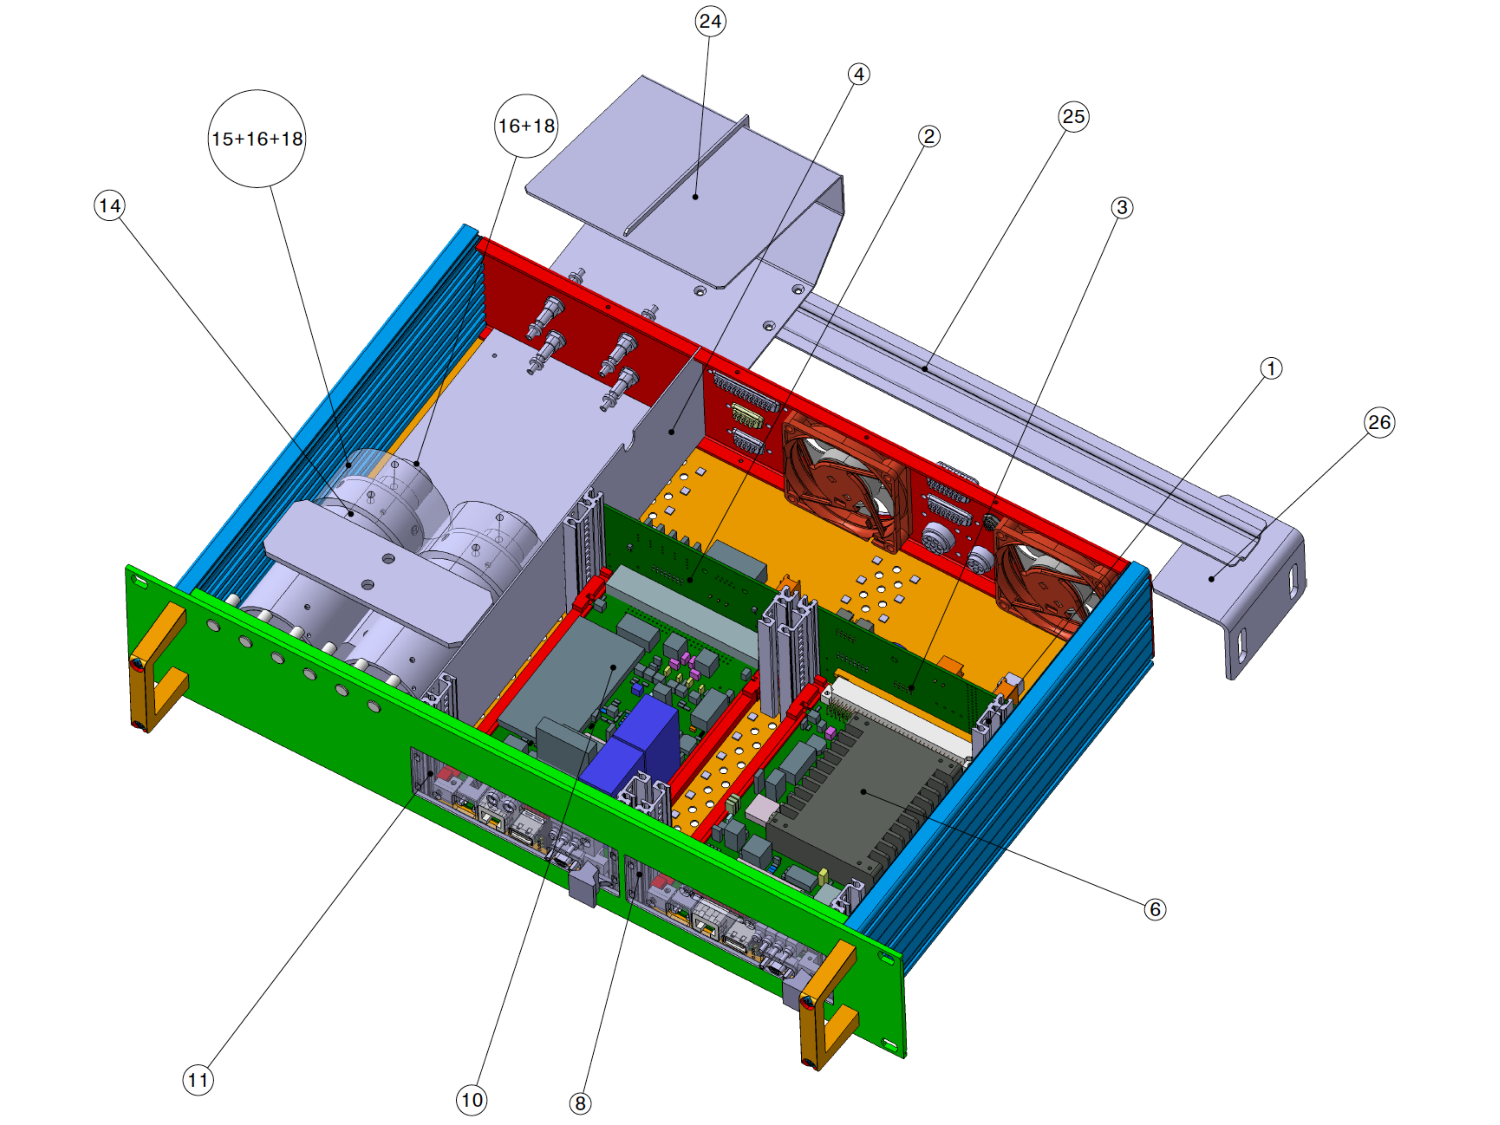
\includegraphics[height=8cm]{figures/pmtbox_meca.pdf}
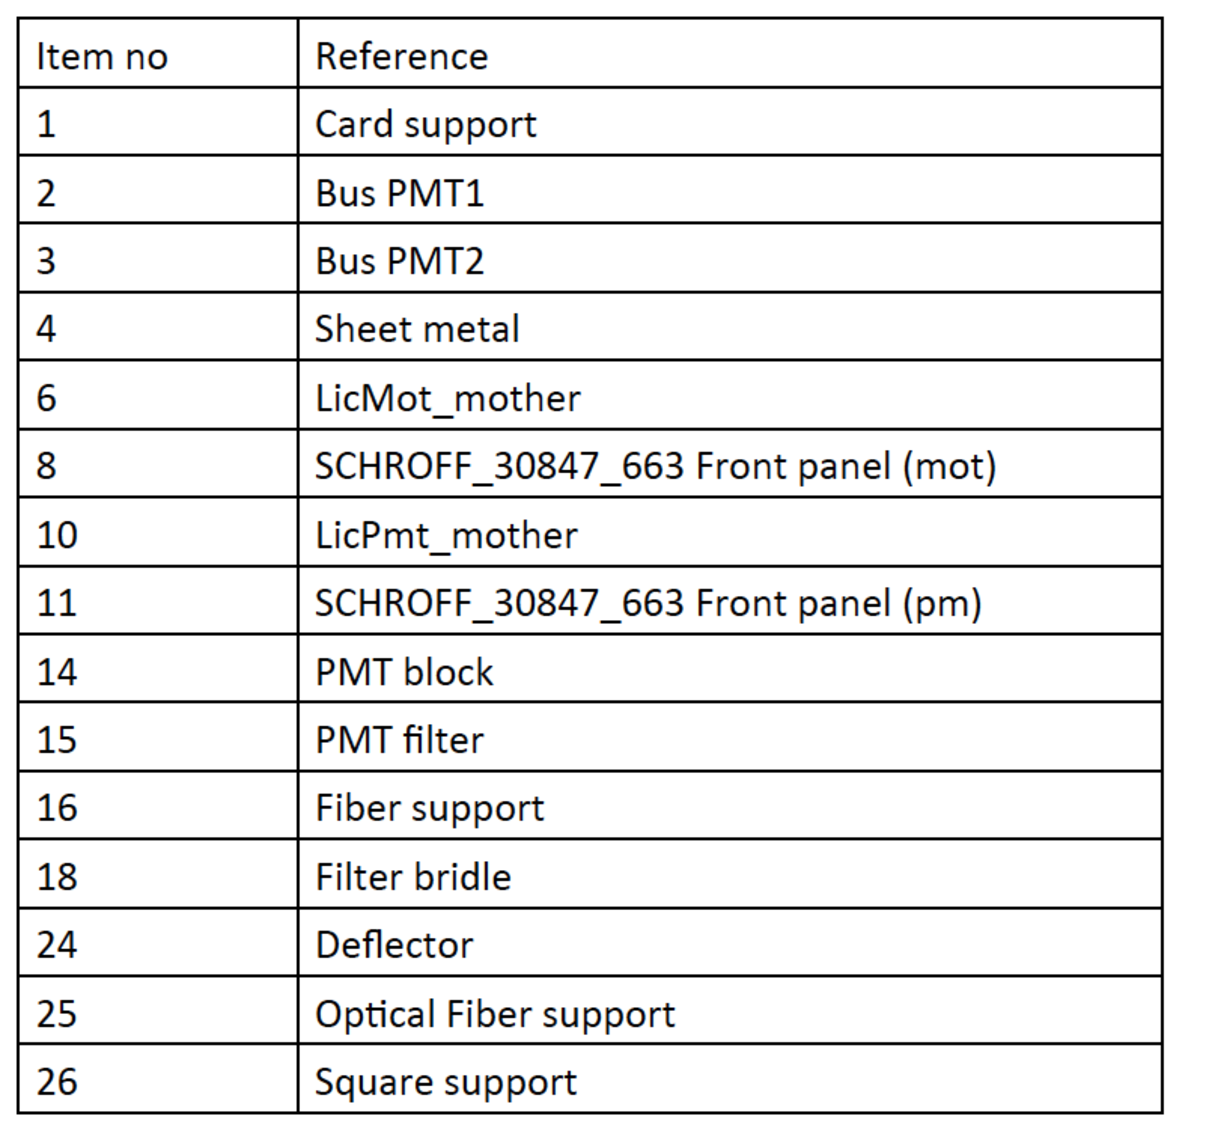
\includegraphics[height=4cm]{figures/pmtbox_list.pdf}
\caption{Schematic of the PMT box.}\label{fig:laspmtbox}
\end{figure}

\begin{itemize}

\item \licpmt (Fig. \ref{fig:laslicpmt}) : this module is used to set the high voltage to the two PMTs located in the box. It provides measurements of temperature and humidity inside of the optics box and is used to manage the interlock chain that prevents users from flashing the \laser~when the optics box is open. \licpmt~is also implied in the configuration and the control of the laser pump (slow control part) and is used to switch the \laser~pump (power supply relay) on. 

\begin{figure}[htbp]
\centering
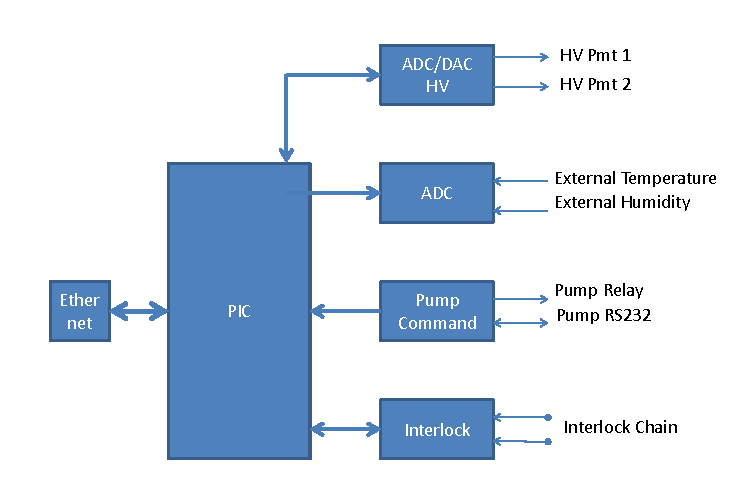
\includegraphics[height=5cm]{figures/licpmt_scheme.pdf}
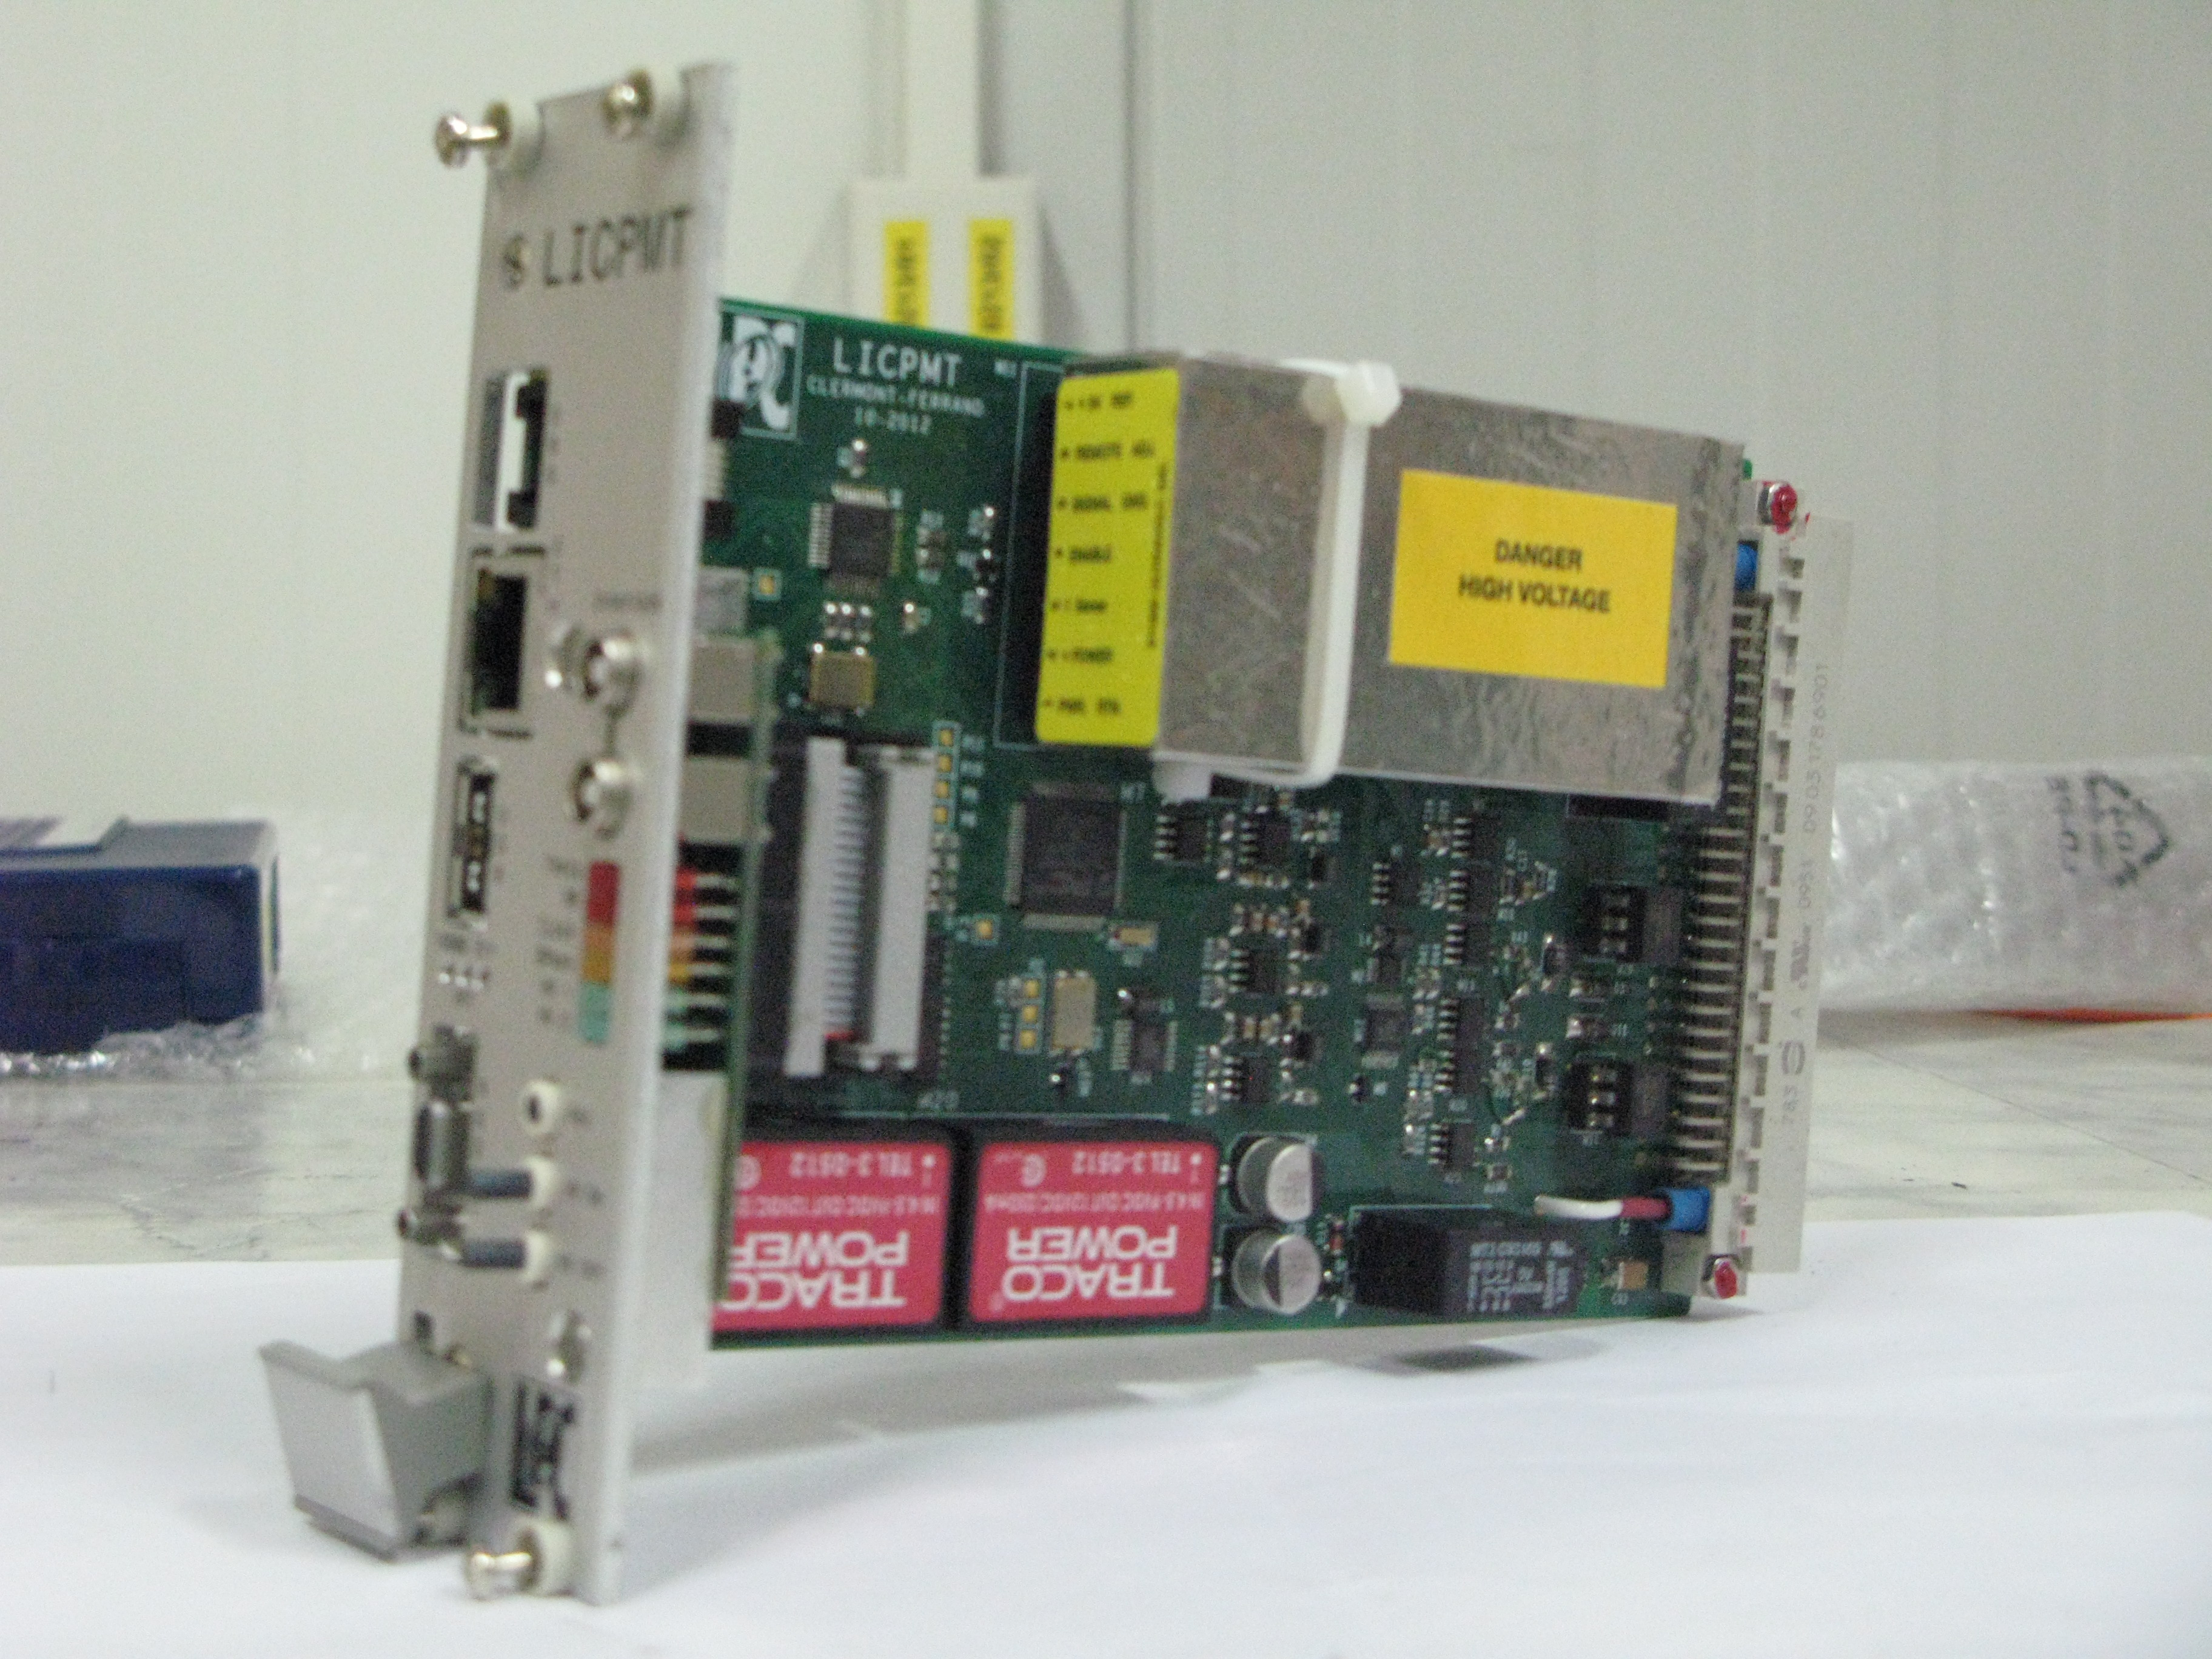
\includegraphics[height=5cm]{figures/licpmt.JPG}
\caption{Schematic (left) and view(right) of the \licpmt~card}\label{fig:laslicpmt}
\end{figure}

\item \licmot~(Fig. \ref{fig:laslicmot}) : this module is used to drive the shutter and the filter wheel located in the optics box. 

\begin{figure}[htbp]
\centering
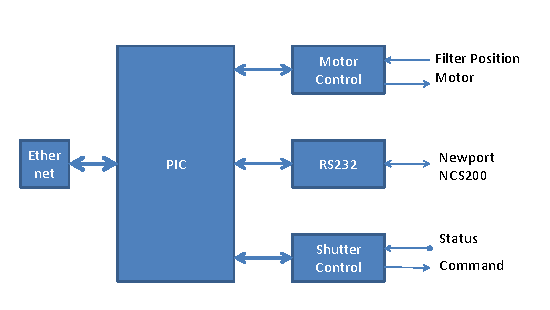
\includegraphics[height=5cm]{figures/licmot_scheme.pdf}
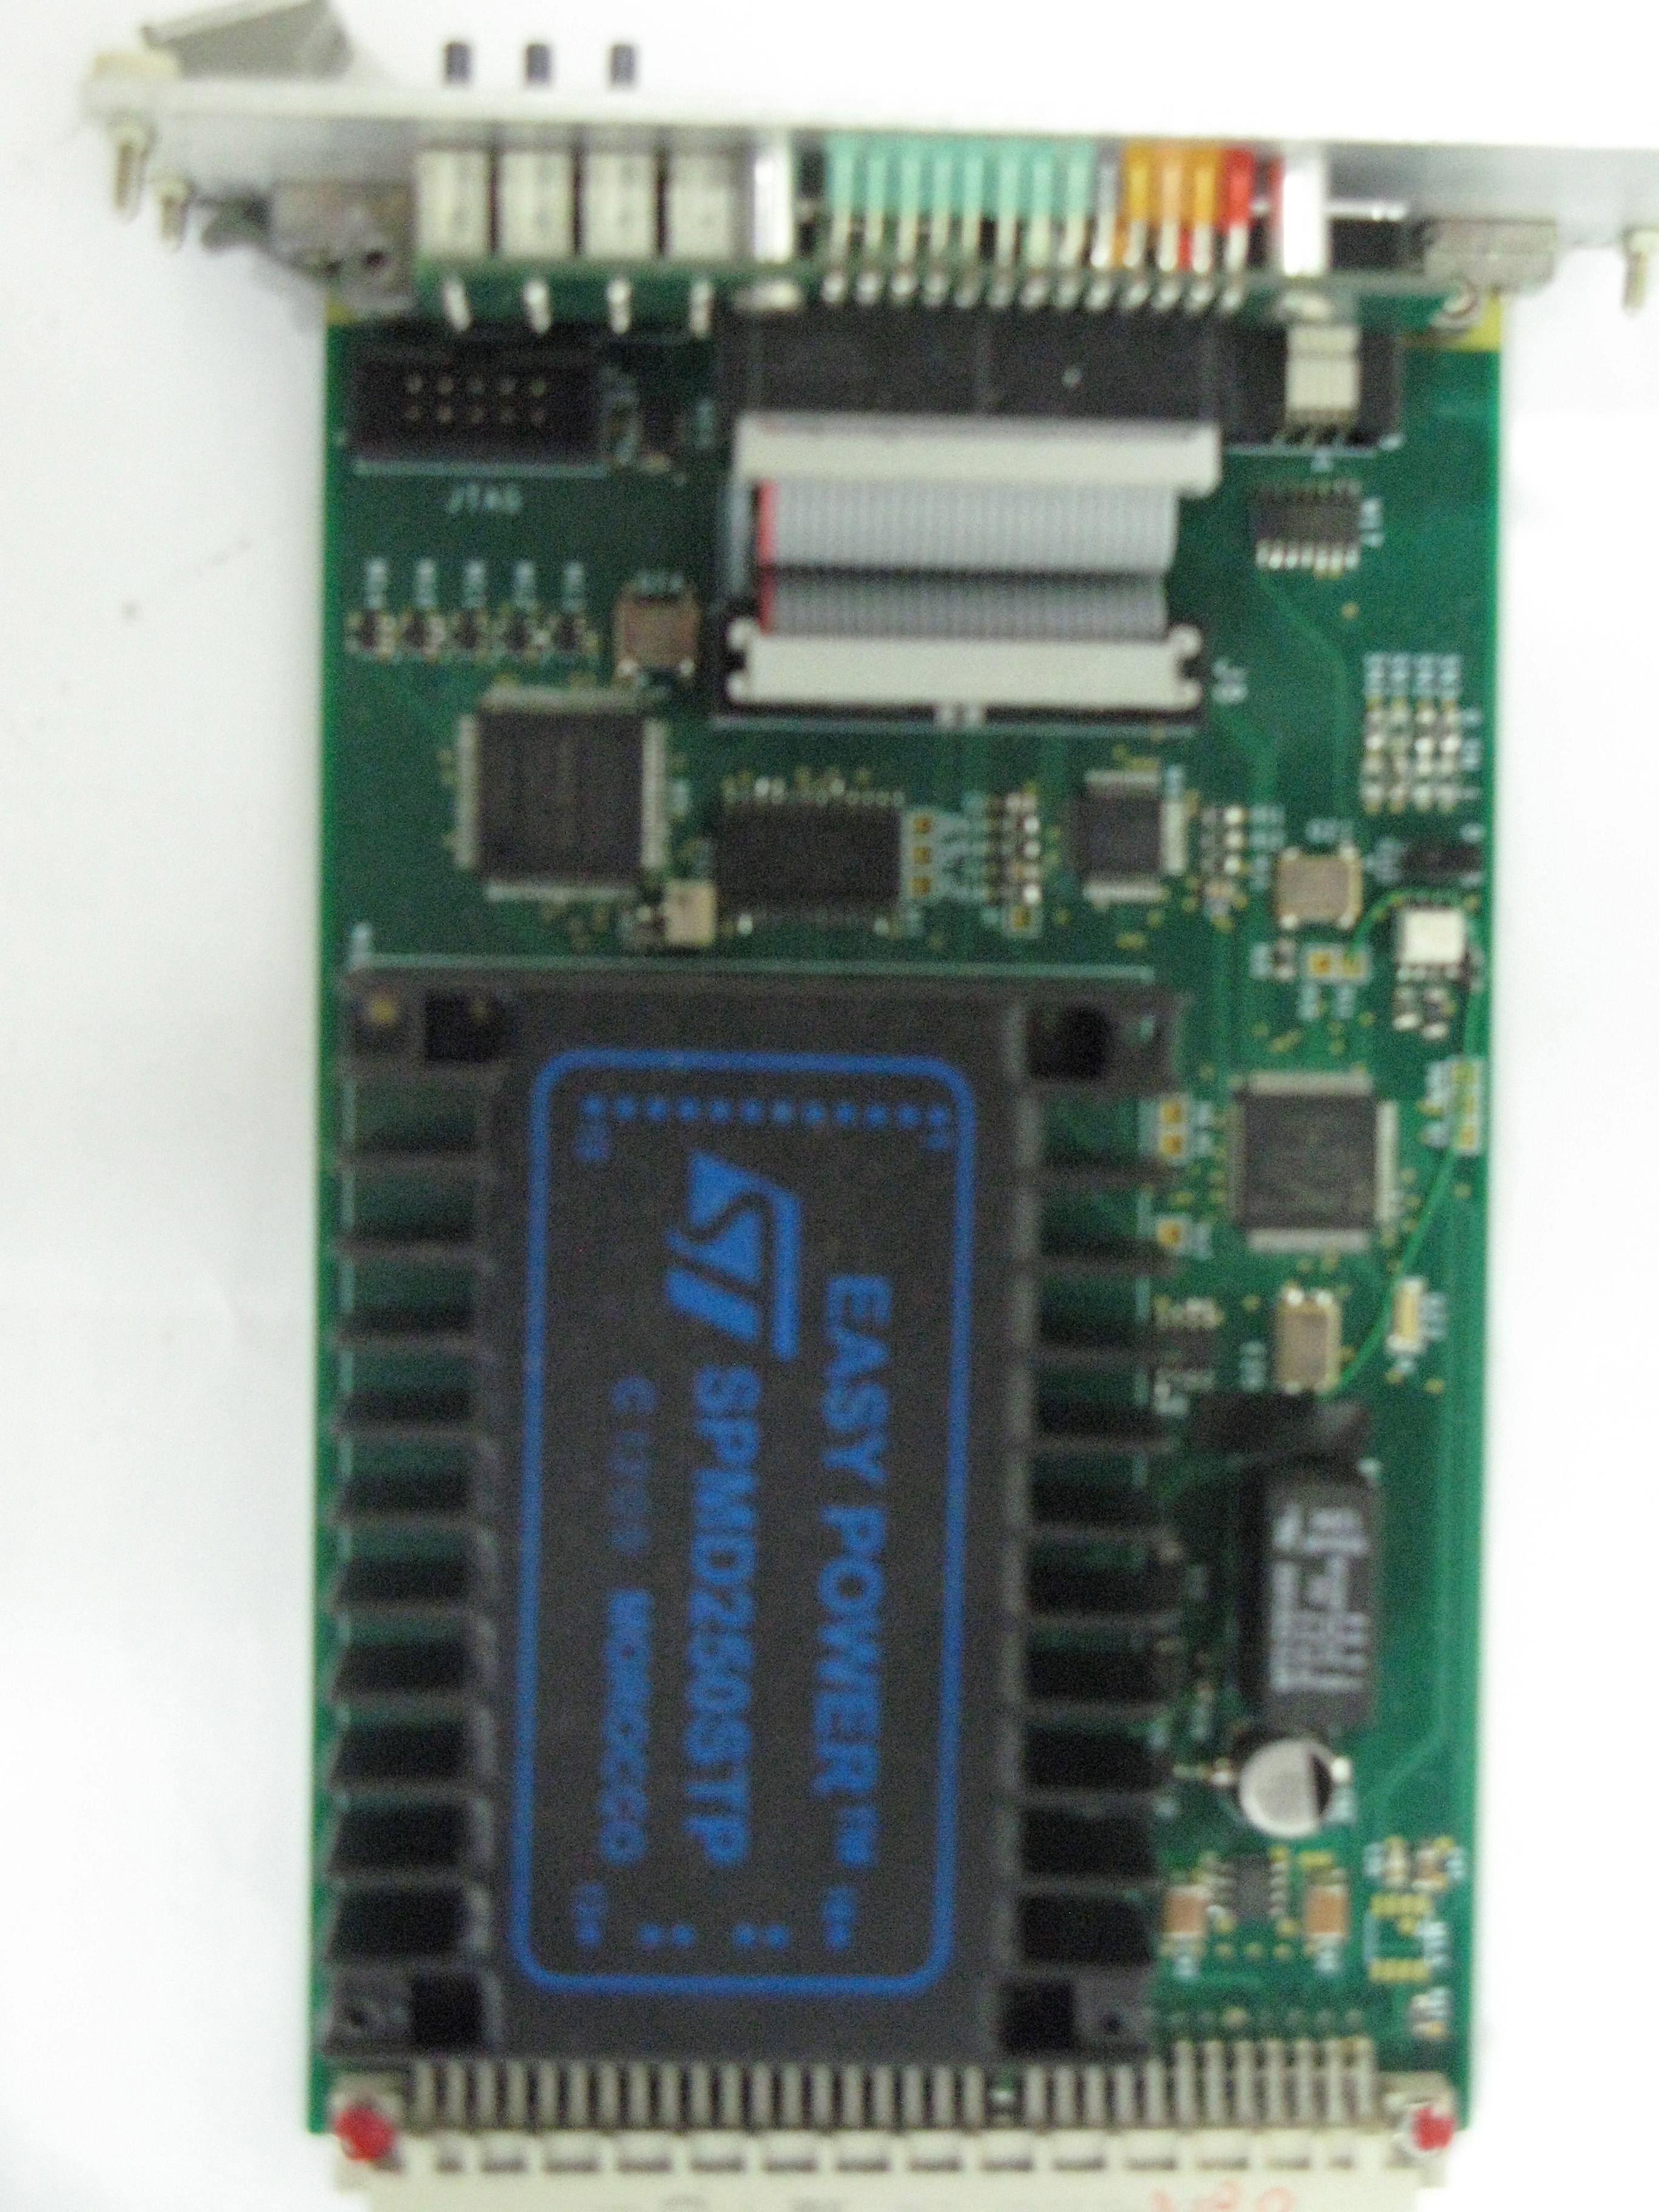
\includegraphics[height=5cm]{figures/licmot.JPG}
\caption{Schematic (left) and view (right) of the \licmot~card}\label{fig:laslicmot}
\end{figure}

\end{itemize}

Two optical fibers are plugged at the rear of the box to transmit the \laser~signal from the optics box to the PMTs. For the same reasons as for the photodiode box (air flow in the USA15 racks for electronics cooling), deflectors have been installed to ensure that the optical fibers are maintained in a stable position.

